\subsection{Errors}
\label{sec:errors}
The collected charge is calculated using \ref{eq:capacitance}, hence
\begin{equation}
  \label{eq:uncertainties}
  \delta Q = \sqrt{(V \delta C)^2 + (C \delta V)^2}.
\end{equation}
The capacitance of the pre-amplifier was given in \autocite{LabInstruction}
without uncertainty so, to be conservative, we will assume $\delta C =
0.5$~pF. The high voltage power supply (HVPS) was used to adjust and read the
input, the sensitivity of the instrument is $\pm$ 1~V, thus $\delta V = 1$~V.

The charge collected in the anode was obtained feeding the input of the
preamplifier with a square pulse and measuring the MCA response.
\begin{equation}
  Q = C V_{p}(n)
\end{equation}
Where Q is the charge collected, the C capacitance and n is the MCA response,
the latter also depends linearly on the gain
\begin{equation}
  V_{p}(n_g) = \alpha_g n_g C + \beta_g
\end{equation}
Hence the error on the collected charge is given by
\begin{equation}
  \delta Q = \sqrt{(\delta C V_p )^2 + \left( C \sqrt{( n_g \delta \alpha_g)^2 +
        (\delta \beta_g)^2} \right)^2 + (C \alpha \delta n_g)^2}.
\end{equation}
For the resolution, the errors are treated and obtained from the Gaussian
distribution
\begin{equation}
  \delta R = \sqrt{\left( \frac{\delta \sigma}{\sigma} \right)^2 + \left(
      \frac{\delta \mu}{\mu} \right)^2}.
\end{equation}
\begin{figure}[!h]
  \centering
  \begin{subfigure}[t]{.48\linewidth}
    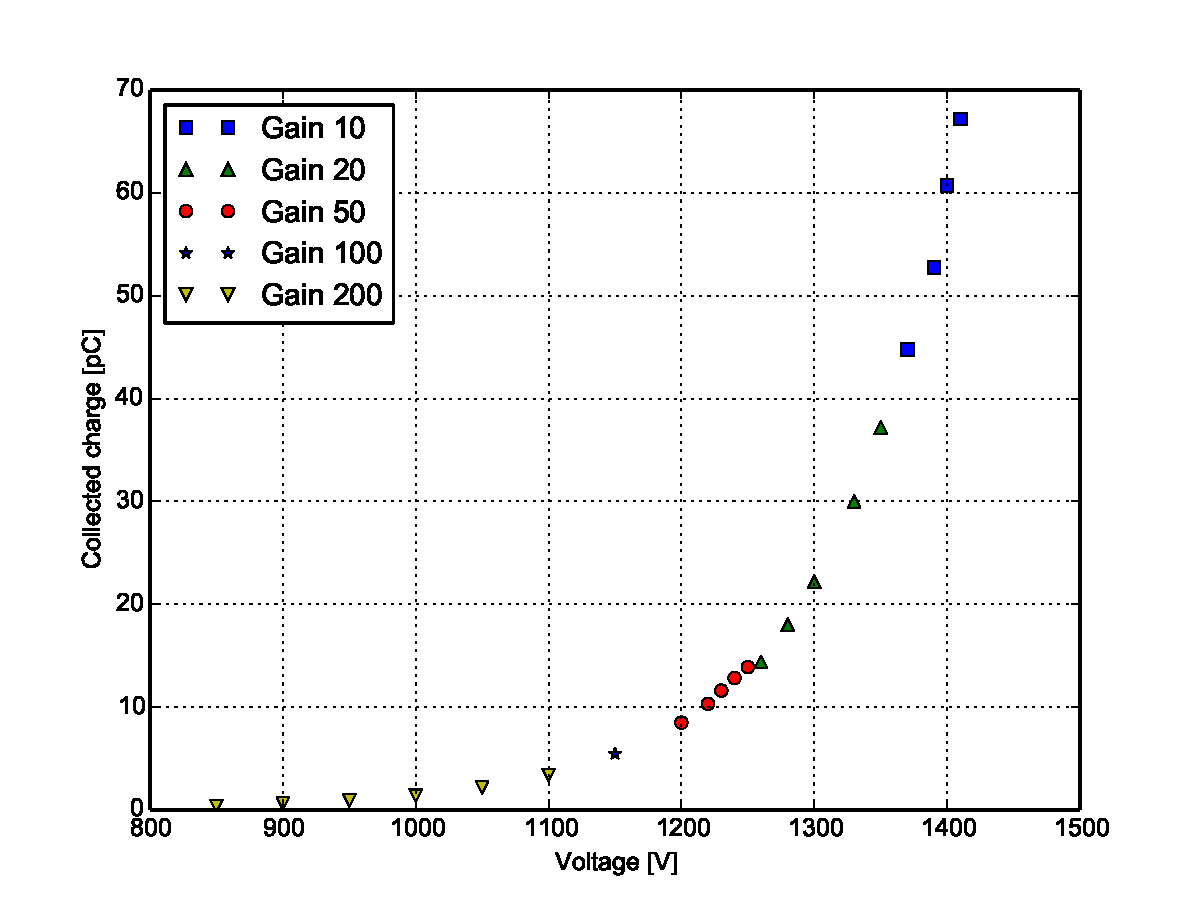
\includegraphics[width=\linewidth]{charge_vs_voltage}
    \caption{}
    \label{fig:charge_vs_voltage}
  \end{subfigure}
  \begin{subfigure}[t]{.48\linewidth}
    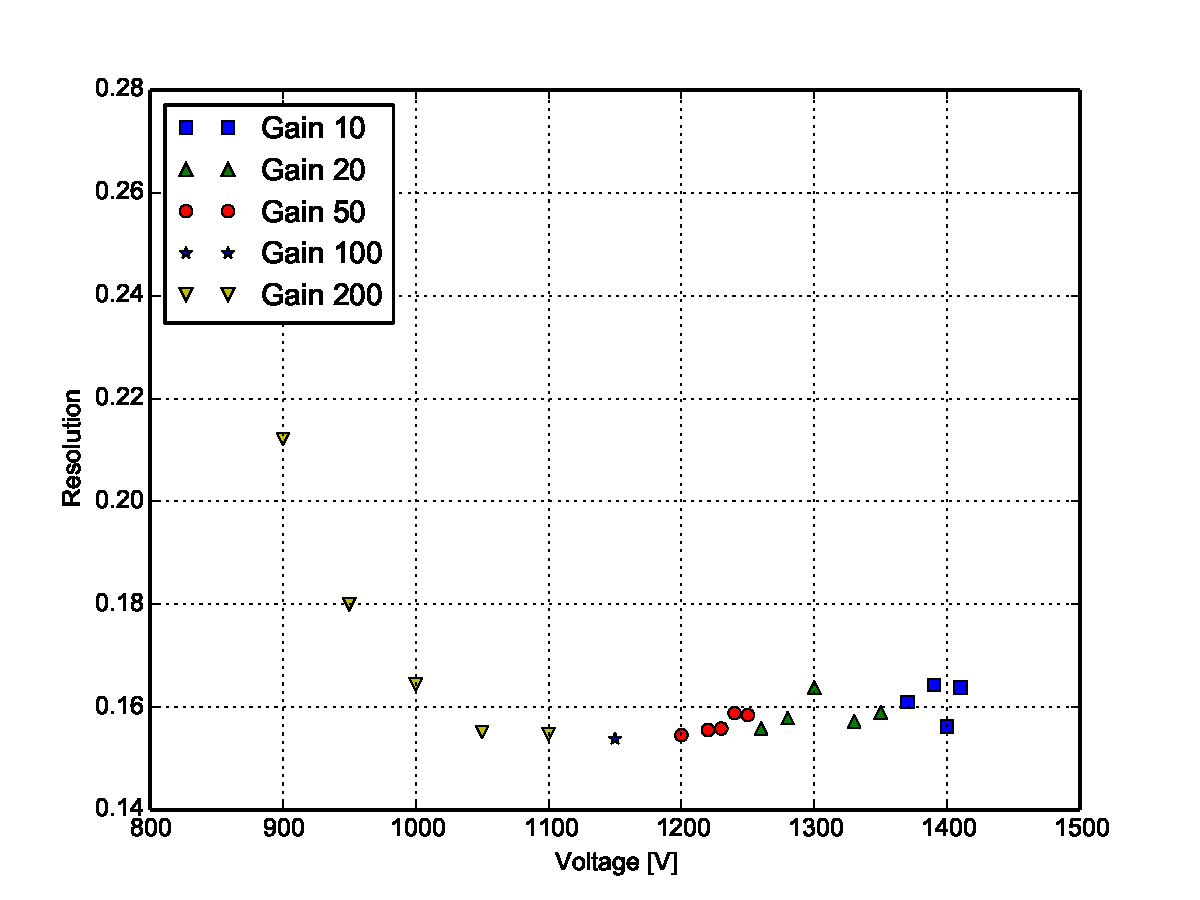
\includegraphics[width=\linewidth]{resolution_vs_voltage}
    \caption{}
    \label{fig:resolution_vs_voltage}
  \end{subfigure}
  \caption{}
  \label{fig:results}
\end{figure}
%%% Local Variables:
%%% mode: latex
%%% TeX-master: "prop_counter"
%%% End:
